\section{Iteración I}
\subsection{Resumen}
En esta iteración se realizó el renderizado de un modelo 3D propio, así como su implementación en la aplicación.
\subsection{Desarrollo}
El renderizado de un modelo 3D se a realizó utilizando la herramienta Blender, en dicha herramienta modelamos una simple capsula, que se exportó en dos tipos de archivos: .obj y .mtl, los cuales convertimos usando Google Sceneform Tools, a un modelo entendible para ARCore. En la figura 4.27 se puede observar el modelo que implementamos.
\begin{figure}[H]
	\centering
	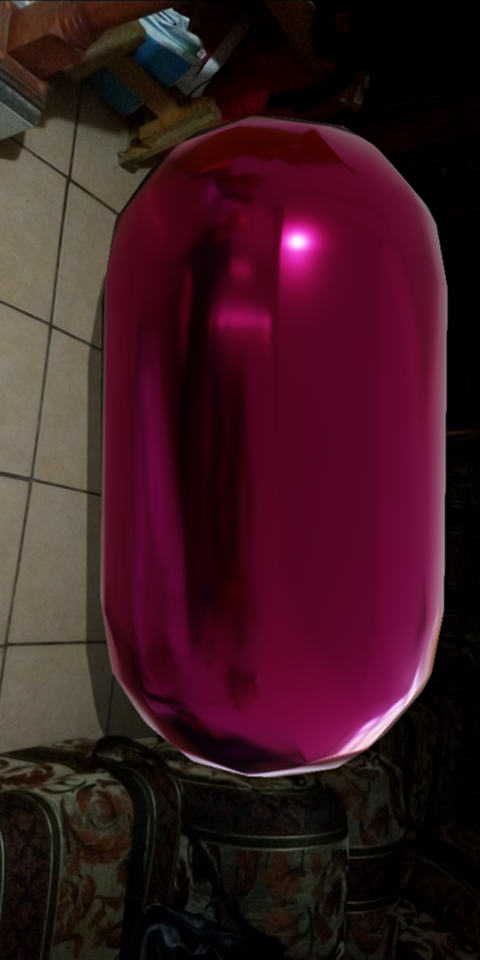
\includegraphics[width=8cm,height=12cm]{imagenes/iteraciones/AR2.png}
	\caption{Primer modelo 3D implementado en ARcore}
	\label{fig:1modelo}
\end{figure} 